\documentclass[]{article}
\usepackage{lmodern}
\usepackage{amssymb,amsmath}
\usepackage{ifxetex,ifluatex}
\usepackage{fixltx2e} % provides \textsubscript
\ifnum 0\ifxetex 1\fi\ifluatex 1\fi=0 % if pdftex
  \usepackage[T1]{fontenc}
  \usepackage[utf8]{inputenc}
\else % if luatex or xelatex
  \ifxetex
    \usepackage{mathspec}
  \else
    \usepackage{fontspec}
  \fi
  \defaultfontfeatures{Ligatures=TeX,Scale=MatchLowercase}
\fi
% use upquote if available, for straight quotes in verbatim environments
\IfFileExists{upquote.sty}{\usepackage{upquote}}{}
% use microtype if available
\IfFileExists{microtype.sty}{%
\usepackage{microtype}
\UseMicrotypeSet[protrusion]{basicmath} % disable protrusion for tt fonts
}{}
\usepackage[margin=1in]{geometry}
\usepackage{hyperref}
\hypersetup{unicode=true,
            pdftitle={Urbanización y modificación de la distribución de especies. Una primera aproximación a la ecología urbana costera.},
            pdfauthor={Giorgia Graells},
            pdfborder={0 0 0},
            breaklinks=true}
\urlstyle{same}  % don't use monospace font for urls
\usepackage{graphicx,grffile}
\makeatletter
\def\maxwidth{\ifdim\Gin@nat@width>\linewidth\linewidth\else\Gin@nat@width\fi}
\def\maxheight{\ifdim\Gin@nat@height>\textheight\textheight\else\Gin@nat@height\fi}
\makeatother
% Scale images if necessary, so that they will not overflow the page
% margins by default, and it is still possible to overwrite the defaults
% using explicit options in \includegraphics[width, height, ...]{}
\setkeys{Gin}{width=\maxwidth,height=\maxheight,keepaspectratio}
\IfFileExists{parskip.sty}{%
\usepackage{parskip}
}{% else
\setlength{\parindent}{0pt}
\setlength{\parskip}{6pt plus 2pt minus 1pt}
}
\setlength{\emergencystretch}{3em}  % prevent overfull lines
\providecommand{\tightlist}{%
  \setlength{\itemsep}{0pt}\setlength{\parskip}{0pt}}
\setcounter{secnumdepth}{0}
% Redefines (sub)paragraphs to behave more like sections
\ifx\paragraph\undefined\else
\let\oldparagraph\paragraph
\renewcommand{\paragraph}[1]{\oldparagraph{#1}\mbox{}}
\fi
\ifx\subparagraph\undefined\else
\let\oldsubparagraph\subparagraph
\renewcommand{\subparagraph}[1]{\oldsubparagraph{#1}\mbox{}}
\fi

%%% Use protect on footnotes to avoid problems with footnotes in titles
\let\rmarkdownfootnote\footnote%
\def\footnote{\protect\rmarkdownfootnote}

%%% Change title format to be more compact
\usepackage{titling}

% Create subtitle command for use in maketitle
\newcommand{\subtitle}[1]{
  \posttitle{
    \begin{center}\large#1\end{center}
    }
}

\setlength{\droptitle}{-2em}
  \title{Urbanización y modificación de la distribución de especies. Una primera
aproximación a la ecología urbana costera.}
  \pretitle{\vspace{\droptitle}\centering\huge}
  \posttitle{\par}
  \author{Giorgia Graells}
  \preauthor{\centering\large\emph}
  \postauthor{\par}
  \predate{\centering\large\emph}
  \postdate{\par}
  \date{4 diciembre 2017}

\setlength{\parindent}{0em}
\setlength{\parskip}{1em}

\begin{document}
\maketitle

\subsection{Introducción}\label{introduccion}

Uno de los principales moduladores de la pérdida de habitat en el
planeta es el cambio de uso de suelo. Esta transformación del habitat ha
sido provocada principalmente por actividades del hombre como la
agricultura, la que incluye el efecto de los cultivos, como también de
la deforestación nativa y reforestación con plantaciones comerciales y
la sobrexplotación de los suelos producto de la ganadería. Sin embargo,
otro factor importante que ha generado cambios aun más dramáticos que la
agricultura, aunque quizás en una menor extensión, es la urbanización.
El factor urbano genera cambios de uso de suelo casi irreversibles a las
condiciones naturales en comparación con la agricultura, que a pesar de
ser más extensiva, mantiene un componente vegetal que puede permitir la
vida silvestre bajo ciertas condiciones.

Una forma en la que se puede observar de forma cuantitativa el cambio o
impacto del hombre es con el llamado \emph{Human Foot Print}, el cual es
un índice que muestra el porcentage de influencia relativa del hombre
sobre cada bioma terrestre del planeta (Sanderson et al. 2002). Los
sitios más afectados y que por lo tanto muestran un mayor porcentaje de
influencia humana son aquellos afectados por la agricultura extensiva y
las zonas urbanas.

Debido a esto último, zonas agrícolas y urbanas han sido blanco de
estudio de cómo los cambios del paisaje o habitat modifican las
comunidades naturales y distribución de las poblaciones. Sin embargo,
alrededor de 30 años atrás, comenzó el estudio de la ecología urbana.
Esta disciplina, que partió centrada en el ser humano y sus
interacciones dentro de la ciudad, con el paso del tiempo se enfocó en
el estudio de las especies que se encontraban viviendo en sitios
urbanizados como parte de su hábitat (Marzluff et al. 2008). A partir de
estos estudios se han podido determinar gradientes de urbanización que
podrían explicar la presencia de especies en lugares que no parecerían
aptos para ellas, viendose modificadas sus distribuciones de rango
natural.

Es importante tomar en cuenta los factores que intervienen para que una
especie se encuentre en el lugar que habita. El año 2011 surge un modelo
en el cual la distribución de especies dependería de \textbf{factores
ábioticos} como el conjunto de condiciones ambientales óptimas en que
una especies pueda sobrevivir y reproducirse, tal como rangos de
temperatura y humedad; los \textbf{factores bióticos} como las
interacciones que una especie puede soportar o incluso necesitar, como
depredación o mutualismos, respectivamente; y la \textbf{migración},
como la dispersión o la posibilidad de una especie de llegar a un lugar
óptimo para asentarse (Peterson 2011).

Considerando que el hombre actúa a la vez como un factor abiótico, por
ejemplo generando nuevas condiciones de temperatura; como un factor
biótico, generando nuevos hábitats para las especies o actuando como
moduladores del comportamiento; o incluso generando barreras de
migración o dispersion de especies, en este ensayo se propone un nuevo
modelo, en el cual el ser humano corresponde a un cuarto factor. El
modelo propuesto considera la interacción de los cuatro factores, en
donde se pueden identificar dos secciones posibles en los cuales las
especies pueden vivir. En un área, las especies necesitarán de ciertas
condiciones abióticas, interacciones bióticas, factores de dispersión y
condiciones de influencia humana para poder vivir (Fig.1, número 2). En
la otra área (Fig.1, número 1), se encuentran las especies que no pueden
vivir bajo hábitats que presentan influencia humana. La influencia
humana puede ser cuantificada por valores de urbanización y por lo tanto
considerada una variable en donde las distribuciones de las especies se
verán modificadas según los diferentes grados de urbanización que
presentan las ciudades.

\begin{figure}
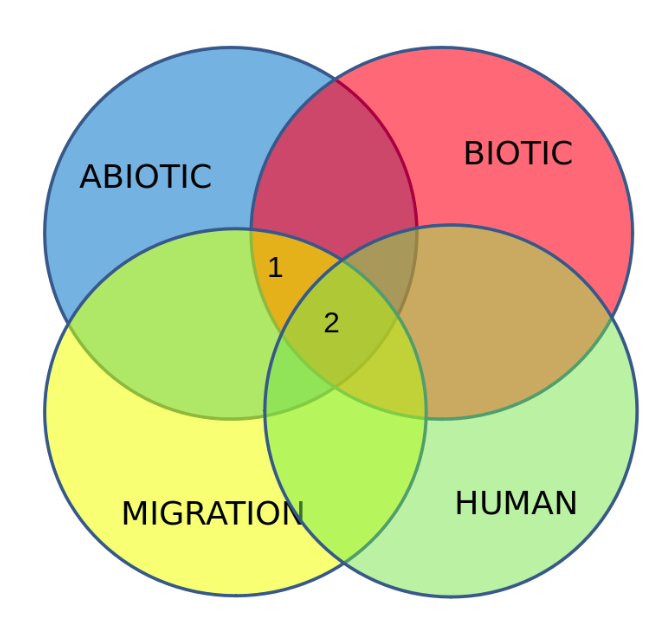
\includegraphics[width=3.34in]{/home/giorgia/Documents/frontera-final/modelodis2} \caption{Modelo propuesto donde el ser humano es un cuarto factor determinante en la distribución de especies. Modificado de Peterson 2011. Los números 1 y 2 corresponden a condiciones en donde las especies pueden vivir, sin y con la influencia del ser humano, respectivamente.}\label{fig:unnamed-chunk-1}
\end{figure}

\subsubsection{Diferencias poblacionales debido a diferencias locales de
temperatura}\label{diferencias-poblacionales-debido-a-diferencias-locales-de-temperatura}

El ser humano través del cambios en el uso del suelo ha sido capaz de
modificar la temperatura local (Chen et al. 2006). El \emph{Urban Heat
Island} (UHI) corresponde al aumento de la temperatura hacia el centro
de las ciudades el cual se va discipando a medida que se va hacia las
afueras de la ciudad (Oke 1973). De esta forma, ciudades de mayor tamaño
poseen mayor diferencia de temperaturas, afectando de distinta forma en
distintos biomas (Imhoff et al. 2010). Este fenómeno ha generado no sólo
cambios de hasta 4°C en la sensación térmica de las personas habitantes
de las ciudades, sino que también sobre las poblaciones naturales que
habitan las ciudades.

Un ejemplo de cómo la variación local de la temperatura provocada por el
UHI modifica la distribución de las especies, lo entrega la especie de
hormiga cortadora de hojas \emph{Atta sexdens} que habita en Sao Paulo
(Angilletta Jr et al. 2007). Colonias urbanas y rurales se encuentran
diferenciadas, en donde las colonias urbanas han demostrado que se
recuperan más rápidamente de shocks térmicos provocados por tempraturas
altas (42°C), en comparación con las colonias rurales que no muestran
adaptaciones a altas temperaturas. Considerando el modelo propuesto
(Fig. 1), la colonia de hormigas urbanas que presentan adaptaciones a
las condiciones de temperatura de la ciudad se encontrarían en el área
2, la colonia no urbana se encontraría en el área 1, donde no soporta
las condiciones con influencia humana.

\subsubsection{El ser humano es capaz de fragmentar el habitat natural y
crear nuevos habitats
artificiales.}\label{el-ser-humano-es-capaz-de-fragmentar-el-habitat-natural-y-crear-nuevos-habitats-artificiales.}

Dentro de las ciudades existen, por lo general, verdaderos mosaicos de
áreas verdes que generan habitats disponibles para especies. Dentro de
esto, es factible ver un gradiente de influencia humana en donde hay
lugares que presentan una saturación de edificación (como el centro de
las ciudades), construcciones, pavimentación en donde las calles poseen
arboles y prados, plazas, parques, e incluso reservas naturales. Así
como las especies poseen distintos requerimientos para vivir, éstas
podrán habitar los distintos espacios dentro de la ciudad utilizando
este gradiente.

En estudios de ecología urbana se ha visto que las especies de aves
presentes en las ciudades frecuentan tipos de habitats ubicados en las
ciudades según este gradiente. De esta forma aves estudiadas en Santa
Clara, CA fueron divididas entre expotadores urbanas, adaptables
suburbanas y aquellas que evitaban los sitios urbanos en base a sus
avistamientos (Blair 1996). Las especies que evitan los sitios
urbanizados deben ser más especialistas en sus requerimientos, los
cuales solo pueden ser encontrados en ambientes más naturales sólo
presentes fuera de las ciudades o en zonas como reservas naturales
dentro de las ciudades (Fig. 1, área 1). Las especies adaptables
suburbanas serán especies más generalistas en base a sus requerimientos,
los cuales pueden ser encontrados en lugares como plazas, parques y
barrios residenciales (Fig. 1, área 1 y 2). Las especies que son
explotadoras urbanas no solo serán especies generalistas capaces de
encontrar sus requerimientos en las ciudades, sino que además las
condiciones de mayor urbanización, la presencia de edificación y
pavimento, deberán presentar considerables ventajas para vivir y
reproducirse (Fig. 1, área 2). En esta ultima categoria caen las palomas
y gorriones, para los cuales la urbanización presentará probablemente
escape a depredadores, facilidad de encontrar alimento y/o facilidad de
nidificación.

\subsubsection{Luz artificial puede generar tanto cambios en el
comportamiento de las especies o actuar como barreras de
dispersión}\label{luz-artificial-puede-generar-tanto-cambios-en-el-comportamiento-de-las-especies-o-actuar-como-barreras-de-dispersion}

La urbanización ha traído un problema a la naturaleza anexo, que
corresponde a la luz artificial. La luz artificial ha generado el cambio
en los ciclos de día-noche tanto para humanos como para el resto de las
especies que habitan las zonas urbanas, sus alrededores o incluso, para
quienes las cruzan, por ejemplo en el vuelo.

Se ha visto que los cambios ciclo día noche a través del efecto de la
luz artificial genera cambios a nivel de comportamiento, modificando los
patrones de alimentación. Un ejemplo de esto es el caso de peces que
viven en las costas de Boston, MA (Bolton et al. 2017). Estos peces de
alimentación diurna y de actividad nocturna (aparecen en mayor cantidad
durante la noche), poseen un comportamiento diurno ante la presencia de
luz artificial durante la noche. El efecto de la luz artificial, más la
actividad durante el día puede generar cambios importantes en la
comunidad. Por un lado los peces pueden ser más facilmente identificados
por depredadores, o incluso, la alimentación nocturna y diurna puede
generar una sobrexplotación del recurso alimenticio sobre el sustrato.

Un segundo ejemplo es el caso de invertebrados terrestres capturados con
trampas pitfall ubicadas entre focos de iluminaria pública (Davies,
Bennie, and Gaston 2012). Bajo estas condiciones, depredadores y
carroñeros muestran cambios en su comportamiento ya que salen más
durante la noche bajo luz artificial que en oscuridad o incluso durante
el día. En este caso como en el anterior, cambios en las redes tróficas
pueden ejercer modificaciones sobre las población, lo cual puede verse
reflejado en la distribución de la especie.

Por otro lado, luz artificial también puede actuar como una barrera para
el movimiento de las especies, como el caso de murciélagos frugívoros
que se ven afectados negativamente (Lewanzik and Voigt 2014). Aunque
también puede ser factor de mortalidad importante. Es así como tortugas
de la especie \emph{Caretta caretta}, que llegan a desovar a las playas
de Florida, se ven desorientadas por la luminaria de la costanera,
pierden el rumbo y son atropelladas (McFarlane 1963). Esta
desorientación se presenta incluso en neonatos de la misma especie
(Simoes 2017). En ambos casos, estas especies presentan problemas en los
hábitats con influencia humana (como los caminos o playas iluminadas),
por lo tanto sus distribuciones estarían determinadas por los factores
que determinan el área 1 de este modelo (Fig. 1).

\subsubsection{Pérdida de habitat a través del cambio de uso de suelo es
un fenomeno gradual que puede permitir la adaptación de las
especies}\label{perdida-de-habitat-a-traves-del-cambio-de-uso-de-suelo-es-un-fenomeno-gradual-que-puede-permitir-la-adaptacion-de-las-especies}

La pérdida de habitat natural es comúnmente un proceso gradual en el
tiempo, en el cual las especies se ven afectadas considerablemnete por
su disminución. Sin embargo, el que algunas especies puedan ser más
plásticas que otras a estos cambios, sumado al tiempo de asimilación de
los cambios, puede generar una mayor adaptación de especies a los nuevos
hábitats.

Un estudio en México da evidencia de este fenómeno de forma tangencial
(Peterson et al. 2006). Peterson y colaboradores el 2006 realizaron
modelaciones de distribución de 11 especies de endémicas de córvidos,
considerando los cambios de uso de suelo desde el año 1976 hasta el
2000. Para esto se analizó la pérdida histórica de la capa vegetal
natural en el país y los cambios de presencia de las especies. De esta
forma se determinó que existen especies que se vieron afectadas por el
camio de uso de suelo, presentando un 12\% de reducción de su población
original. Otras especies no eran afectadas por el cambio de habitat,
incluso \emph{Cyanolyca nana} no presentó cambios entre su poblacion
original y la del 2000.

\subsubsection{Puesta a prueba: la urbanización como un factor que
modifica la distribución de las
especies}\label{puesta-a-prueba-la-urbanizacion-como-un-factor-que-modifica-la-distribucion-de-las-especies}

Considerando al ser humano como un factor más que determina la
distribución de las especies, se consideró la urbanización como una
variable continua. Se seleccionaron siete especies marinas que habitan
la costa de Chile, se obtuvo sus puntos de presencia por GBIF y se
descargó un mapa de urbanización de Chile (Tuanmu and Jetz 2014). Para
cada una de las especies, se correlacionó cada punto de presencia con el
porcentaje de urbanización que presentaba.

Los resultados indican que todas las especies muestran una mayor
ocurrencia en lugares con baja urbanización. Sin embargo, existen dos
grupos que presentan distintas afinidades por la urbanización: 1.
Aquellas especies en donde la mayor ocurrencia se presenta en lugares
con una urbanización menor al 5\%, en donde se distinguen \emph{Otaria
flavescens} y \emph{Mirounga leonina} (Fig. 1, área 1), y 2. Aquellas
especies que muestran presencias en sitios hasta con 100\% de
urbanización y picks de individuos entre los 0 y 40\% de urbanización,
en donde se distinguen a \emph{Larus dominicanus} y \emph{Phalacrocorax
brasilianus} (Fig. 1, área 2).

A pesar de que este ejercicio debe ser realizado con mayor detalle, en
donde se consideren puntos de presencias reales de avistamiento de las
especies, se puede concluir de forma preliminar que la presencia de
especies se estaría viendo modificada por el porcentaje de urbanización
en la costa.

\subsection{Conclusión}\label{conclusion}

Los efectos del ser humano han ido incrementando con el tiempo. En algún
momento, cuando vivía en grupos pequeños de cazadores recolectores, su
efecto sobre el resto de las especies era netamente trófico. Hoy en día,
el ser humano es más que un depredador y se le ha definido como un
ingeniero ecosistémico ya que modifica los ambientes donde habita. Sin
embargo, los efectos del hombre van más alla del cambio del uso de
suelo, son cambios bióticos, abióticos e incluso ha generado barreras de
dispersión de especies. Es por esto que puede ser considerado como un
cuarto factor en el modelo de los factores que determinan la
distribución de especies, ya que su impacto va má alla de los otros tres
factores por separado.

\subsection*{Referencias}\label{referencias}
\addcontentsline{toc}{subsection}{Referencias}

\hypertarget{refs}{}
\hypertarget{ref-angilletta2007urban}{}
Angilletta Jr, Michael J, Robbie S Wilson, Amanda C Niehaus, Michael W
Sears, Carlos A Navas, and Pedro L Ribeiro. 2007. ``Urban Physiology:
City Ants Possess High Heat Tolerance.'' \emph{PLoS One} 2 (2). Public
Library of Science: e258.

\hypertarget{ref-blair1996land}{}
Blair, Robert B. 1996. ``Land Use and Avian Species Diversity Along an
Urban Gradient.'' \emph{Ecological Applications} 6 (2). Wiley Online
Library: 506--19.

\hypertarget{ref-bolton2017coastal}{}
Bolton, D, M Mayer-Pinto, GF Clark, KA Dafforn, WA Brassil, A Becker,
and EL Johnston. 2017. ``Coastal Urban Lighting Has Ecological
Consequences for Multiple Trophic Levels Under the Sea.'' \emph{Science
of the Total Environment} 576. Elsevier: 1--9.

\hypertarget{ref-chen2006remote}{}
Chen, Xiao-Ling, Hong-Mei Zhao, Ping-Xiang Li, and Zhi-Yong Yin. 2006.
``Remote Sensing Image-Based Analysis of the Relationship Between Urban
Heat Island and Land Use/Cover Changes.'' \emph{Remote Sensing of
Environment} 104 (2). Elsevier: 133--46.

\hypertarget{ref-davies2012street}{}
Davies, Thomas W, Jonathan Bennie, and Kevin J Gaston. 2012. ``Street
Lighting Changes the Composition of Invertebrate Communities.''
\emph{Biology Letters}. The Royal Society, rsbl20120216.

\hypertarget{ref-imhoff2010remote}{}
Imhoff, Marc L, Ping Zhang, Robert E Wolfe, and Lahouari Bounoua. 2010.
``Remote Sensing of the Urban Heat Island Effect Across Biomes in the
Continental Usa.'' \emph{Remote Sensing of Environment} 114 (3).
Elsevier: 504--13.

\hypertarget{ref-lewanzik2014artificial}{}
Lewanzik, Daniel, and Christian C Voigt. 2014. ``Artificial Light Puts
Ecosystem Services of Frugivorous Bats at Risk.'' \emph{Journal of
Applied Ecology} 51 (2). Wiley Online Library: 388--94.

\hypertarget{ref-marzluff2008international}{}
Marzluff, John M, Eric Shulenberger, Wilfried Endlicher, Marina Alberti,
Gordon Bradley, Clare Ryan, U Simon, and ZumBrunnen C Urban Ecology.
2008. \emph{An International Perspective on the Interactions Between
Humans and Nature}. Springer.

\hypertarget{ref-mcfarlane1963disorientation}{}
McFarlane, Robert W. 1963. ``Disorientation of Loggerhead Hatchlings by
Artificial Road Lighting.'' \emph{Copeia} 1963 (1): 153.

\hypertarget{ref-oke1973city}{}
Oke, Tim R. 1973. ``City Size and the Urban Heat Island.''
\emph{Atmospheric Environment (1967)} 7 (8). Elsevier: 769--79.

\hypertarget{ref-peterson2011ecological}{}
Peterson, A Townsend. 2011. \emph{Ecological Niches and Geographic
Distributions (Mpb-49)}. 49. Princeton University Press.

\hypertarget{ref-peterson2006tracking}{}
Peterson, A Townsend, Victor Sanchez-Cordero, Enrique Martínez-Meyer,
and Adolfo G Navarro-Sigüenza. 2006. ``Tracking Population Extirpations
via Melding Ecological Niche Modeling with Land-Cover Information.''
\emph{Ecological Modelling} 195 (3). Elsevier: 229--36.

\hypertarget{ref-sanderson2002human}{}
Sanderson, Eric W, Malanding Jaiteh, Marc A Levy, Kent H Redford,
Antoinette V Wannebo, and Gillian Woolmer. 2002. ``The Human Footprint
and the Last of the Wild.'' \emph{BioScience} 52 (10). BioOne: 891--904.

\hypertarget{ref-SIMOES2017}{}
Simoes, Arley Candido da AND Moura, Thyara Noely AND Silva. 2017.
``Influence of artificial lights on the orientation of hatchlings of
Eretmochelys imbricata in Pernambuco, Brazil.'' \emph{Zoologia
(Curitiba)} 34 (00). scielo.
\url{http://www.scielo.br/scielo.php?script=sci_arttext\&pid=S1984-46702017000100308\&nrm=iso}.

\hypertarget{ref-tuanmu2014global}{}
Tuanmu, Mao-Ning, and Walter Jetz. 2014. ``A Global 1-Km Consensus
Land-Cover Product for Biodiversity and Ecosystem Modelling.''
\emph{Global Ecology and Biogeography} 23 (9). Wiley Online Library:
1031--45.


\end{document}
